

\tikzset{every picture/.style={line width=0.75pt}} %set default line width to 0.75pt        

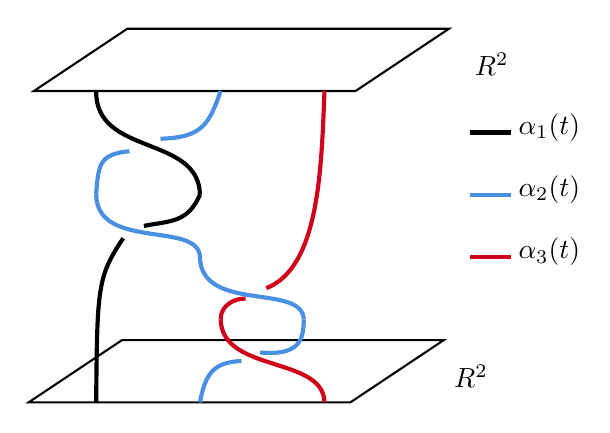
\begin{tikzpicture}[x=0.75pt,y=0.75pt,yscale=-1,xscale=1]
%uncomment if require: \path (0,877); %set diagram left start at 0, and has height of 877

%Shape: Rectangle [id:dp23975536104774442] 
\draw   (205,60) -- (360,60) -- (315,90) -- (160,90) -- cycle ;
%Shape: Rectangle [id:dp4742593007559085] 
\draw   (202.5,210) -- (357.5,210) -- (312.5,240) -- (157.5,240) -- cycle ;
%Curve Lines [id:da2338350605887748] 
\draw [line width=1.5]    (190,90) .. controls (189.5,121.5) and (239.5,111) .. (240,140) ;
%Curve Lines [id:da6958858637133809] 
\draw [color={rgb, 255:red, 74; green, 144; blue, 226 }  ,draw opacity=1 ][line width=1.5]    (250,90) .. controls (244.5,105.5) and (241.5,112.5) .. (221,113) ;
%Curve Lines [id:da1801674192268512] 
\draw [color={rgb, 255:red, 74; green, 144; blue, 226 }  ,draw opacity=1 ][line width=1.5]    (206,119) .. controls (192,120.5) and (191,124.5) .. (190,140) ;
%Curve Lines [id:da04494480422128411] 
\draw [color={rgb, 255:red, 74; green, 144; blue, 226 }  ,draw opacity=1 ][line width=1.5]    (190,140) .. controls (190.5,167) and (239.5,152.5) .. (240,170) ;
%Curve Lines [id:da9002028899774802] 
\draw [color={rgb, 255:red, 74; green, 144; blue, 226 }  ,draw opacity=1 ][line width=1.5]    (240,170) .. controls (240.5,197) and (289.5,182.5) .. (290,200) ;
%Curve Lines [id:da7520709988799963] 
\draw [line width=1.5]    (213,155) .. controls (226,152.5) and (234,153.5) .. (240,140) ;
%Curve Lines [id:da5137431769322998] 
\draw [line width=1.5]    (190,240) .. controls (190.5,185) and (190.5,179.5) .. (203,161) ;
%Curve Lines [id:da2225388746369933] 
\draw [color={rgb, 255:red, 208; green, 2; blue, 27 }  ,draw opacity=1 ][line width=1.5]    (250,200) .. controls (250.5,226) and (299.5,217.5) .. (300,240) ;
%Curve Lines [id:da19326513425460334] 
\draw [color={rgb, 255:red, 74; green, 144; blue, 226 }  ,draw opacity=1 ][line width=1.5]    (240,240) .. controls (243,223.5) and (248.5,221) .. (260,220) ;
%Curve Lines [id:da40134196403228717] 
\draw [color={rgb, 255:red, 74; green, 144; blue, 226 }  ,draw opacity=1 ][line width=1.5]    (290,200) .. controls (290,210.5) and (287.5,217.5) .. (269,216) ;
%Curve Lines [id:da665280040996851] 
\draw [color={rgb, 255:red, 208; green, 2; blue, 27 }  ,draw opacity=1 ][line width=1.5]    (250,200) .. controls (250,193.5) and (256,190) .. (262,190) ;
%Curve Lines [id:da46296116559591394] 
\draw [color={rgb, 255:red, 208; green, 2; blue, 27 }  ,draw opacity=1 ][line width=1.5]    (272,185) .. controls (297.5,175) and (298.5,127.5) .. (300,90) ;
%Straight Lines [id:da17288821057020853] 
\draw [line width=1.5]    (370,110) -- (390,110) ;
%Straight Lines [id:da7810709935908421] 
\draw [color={rgb, 255:red, 74; green, 144; blue, 226 }  ,draw opacity=1 ][line width=1.5]    (370,140) -- (390,140) ;
%Straight Lines [id:da4526710696777342] 
\draw [color={rgb, 255:red, 208; green, 2; blue, 27 }  ,draw opacity=1 ][line width=1.5]    (370,170) -- (390,170) ;

% Text Node
\draw (371,70.4) node [anchor=north west][inner sep=0.75pt]    {$\mathbb{R}^{2}$};
% Text Node
\draw (361,220.4) node [anchor=north west][inner sep=0.75pt]    {$\mathbb{R}^{2}$};
% Text Node
\draw (392,99.4) node [anchor=north west][inner sep=0.75pt]    {$\alpha _{1}( t)$};
% Text Node
\draw (392,129.4) node [anchor=north west][inner sep=0.75pt]    {$\alpha _{2}( t)$};
% Text Node
\draw (392,159.4) node [anchor=north west][inner sep=0.75pt]    {$\alpha _{3}( t)$};


\end{tikzpicture}
